\section{Цель работы}
Цеь работы -- изучить численные методы решения нелинейных уравнений и их
систем, найти корни заданного нелинейного уравнения/системы нелинейных уравнений,
выполнить программную реализацию методов.

\section{Рабочие формулы используемых методов}
\begin{itemize}
	\item Метод хорд \[ x_i = \frac{a_i f(b_i) - b_i f(a_i)}{f(b_i) - f(a_i)} \]
	\item Метод простых итераций \[ x_{i+1} = \varphi(x_i) \]
	\item Метод Ньютона \[ x_i = x_{i-1} - \frac{f(x_{i-1})}{f'(x_{i-1})} \]
	\item Метод простых итераций для решение систем \[ \vec X_{i+1} = \varphi (\vec X_{i}) \]
	\item Метод Ньютона для решения систем \[ x_{i+1} = x_i + \Delta x, y_{i+1} = y_i + \Delta y \]
	      где \( \Delta x, \Delta y \) находятся решением системы
	      \[ J(x,y) \cdot (\Delta x, \Delta y)^T = - (f(x,y), g(x,y))^T \]
\end{itemize}

% 2 5 3
\section{Вычислительная часть задачи}
\subsection{Решение нелинейного уравнения}
\begin{enumerate}
	\item Отделить корни заданного нелинейного уравнения графически (вид уравнения представлен в табл. 6)
	\item Определить интервалы изоляции корней.
	\item Уточнить корни нелинейного уравнения (см. табл. 6) с точностью $\varepsilon = 10^{-2}$.
	\item Используемые методы для уточнения каждого из 3-х корней многочлена представлены в таблице 7.
	\item Вычисления оформить в виде таблиц (1-5), в зависимости от заданного метода. Для всех значений в таблице удержать 3 знака после запятой.
	\item Для метода хорд заполнить таблицу 2.
	\item Для метода Ньютона заполнить таблицу 3.
	\item Для метода простой итерации заполнить таблицу 5. Проверить условие сходимости метода на выбранном интервале.
	\item Заполненные таблицы отобразить в отчете.
\end{enumerate}

Уравнение:
\[
	5.74 x^3 - 2.95 x^2 - 10.28 x - 3.23
\]

График уравнения доступен по ссылке \url{https://www.desmos.com/calculator/6je61ivycq}.
У уравнения есть три корня.
Начальные интервалы изоляции:
\[
	a_1 = -0.9; b_1 = -0.8
	\qquad
	a_2 = -0.4; b_2 = -0.3
	\qquad
	a_3 = 1.7; b_3 = 1.8
\]

\begin{table}[H]
	% \usepackage{tabularray}
	\begin{longtblr}[
		label = none,
		entry = none,
		]{
		width = \linewidth,
		colspec = {Q[58]Q[58]Q[58]Q[56]Q[112]Q[112]Q[108]Q[113]},
		hlines,
		vlines,
		}
		\textnumero & a     & b   & x     & f(a)   & f(b)  & f(x)   & $|x_{k+1} - x_k|$ \\
		1           & 1.7   & 1.8 & 1.732 & -1.031 & 2.184 & -0.059 & --                \\
		2           & 1.732 & 1.8 & 1.734 & -0.059 & 2.184 & -0.003 & 0.002 < 0.01      \\
	\end{longtblr}
	\caption{Решение методом хорд}
\end{table}

$f' = 17.22 x^2 - 5.9 x - 10.28$.
$f'(-0.9) = 8.9782$.
$f'(-0.8) = 5.4608$.
$\lambda = - \frac{1}{8.9782}$.
$\varphi(x) = x - \frac{1}{8.9782} f(x)$.

\begin{table}[H]
	% \usepackage{tabularray}
	\begin{longtblr}[
		label = none,
		entry = none,
		]{
		width = \linewidth,
		colspec = {Q[106]Q[104]Q[100]Q[104]Q[113]},
		hlines,
		vlines,
		}
		\textnumero & $x_k$  & $x_{k+1}$ & $f(x_{k+1})$ & $|x_{k+1} - x_k|$ \\
		1           & -0.9   & -0.839    & -0.018       & 0.061             \\
		2           & -0.839 & -0.831    & -0.018       & -0.008 < 0.01
	\end{longtblr}
	\caption{Решение методом простых итераций}
\end{table}

Для центрального корня
$a_2 = -0.4, b_2 = -0.3$.

% \usepackage{tabularray}
\begin{table}[H]
	\begin{longtblr}[
		label = none,
		entry = none,
		]{
		width = \linewidth,
		colspec = {Q[112]Q[108]Q[108]Q[108]Q[108]Q[227]},
		hlines,
		vlines,
		}
		\textnumero & $x_k$ & $f(x_k)$ & $f'(x_k)$ & $x_{k+1}$ & $|x_{k+1}-x_k|$ \\
		1           & -0.4  & 0.043    & -5.165    & -0.392    & 0.008 < 0.01    \\
	\end{longtblr}
	\caption{Решение метдом Ньютона}
\end{table}

\subsection{Решение системы уравнений}
\[
	\begin{cases}
		y - \cos x = 2 \\
		x + \cos(y-1) = 0.8
	\end{cases}
\]
Метод простой итерации.
График системы представлен по ссылке \url{https://www.desmos.com/calculator/sutbmcle3l}.
Видно, что ответ лежит в пределах:
\[
	0.5 < x < 1 \qquad 2.6 < y < 2.8
\]

Выразим \(x, y\):
\[
	\begin{cases}
		x = 0.8 - \cos (y-1) \\
		y = 2 + \cos x
	\end{cases}
\]

\[
	\varphi(x, y) = ( 0.8 - \cos y, 2 + \cos x )
\]
\[
	\varphi'(x,y) = \begin{bmatrix}
		0         & \sin(y) \\
		- \sin(x) & 0
	\end{bmatrix}
\]

Значение \(\sin(x)\) на \((0.5, 1)\) меняется в пределах от \(0.479\) до $0.841$,
\(\sin(y)\) на $(2.6, 2.8)$ --- от $0.516$ до $0.335$.
Значит итерационный процесс сходится.

\begin{table}[H]
	\centering
	\begin{tabular}{|c | c|}
		\hline
		$x$      & $y$      \\
		\hline
		$0.5$    & $2.6$    \\
		1.656889 & 2.877583 \\
		1.765351 & 1.914014 \\
		1.136519 & 1.806670 \\
		1.033693 & 2.420755 \\
		1.551253 & 2.511650 \\
		1.608061 & 2.019542 \\
		1.233836 & 1.962744 \\
		1.181989 & 2.330620 \\
		1.488794 & 2.379085 \\
		1.523106 & 2.081911 \\
		1.289149 & 2.047672 \\
		1.259006 & 2.277938 \\
		1.449663 & 2.306763 \\
		1.471304 & 2.120837 \\
		1.322722 & 2.099328 \\
		1.304266 & 2.245538 \\
		1.424696 & 2.263386 \\
		1.438532 & 2.145582 \\
		1.343655 & 2.131879 \\
		1.332103 & 2.225194 \\
		1.408681 & 2.236433 \\
		1.417560 & 2.161406 \\
		1.356868 & 2.152637 \\
		1.349563 & 2.212301 \\
		1.398401 & 2.219433 \\
		1.404101 & 2.171542 \\
		1.365258 & 2.165925 \\
		1.360615 & 2.204094 \\
		1.391806 & 2.208637 \\
		1.395462 & 2.178036 \\
		1.370603 & 2.174437 \\
		1.367644 & 2.198859 \\
		1.387578 & 2.201758 \\
		1.389922 & 2.182195 \\
		1.374013 & 2.179890 \\
		1.372124 & 2.195516 \\
		1.384870 & 2.197368 \\
		1.386371 & 2.184857 \\
		1.376191 & 2.183382 \\
		1.374985 & 2.193379 \\
		\hline
	\end{tabular}
\end{table}

\section{Программная часть задачи}
\inputminted[breaklines]{Python}{./solution/equation.py}
\inputminted[breaklines]{Python}{./solution/system.py}

\begin{figure}[H]
	\centering
	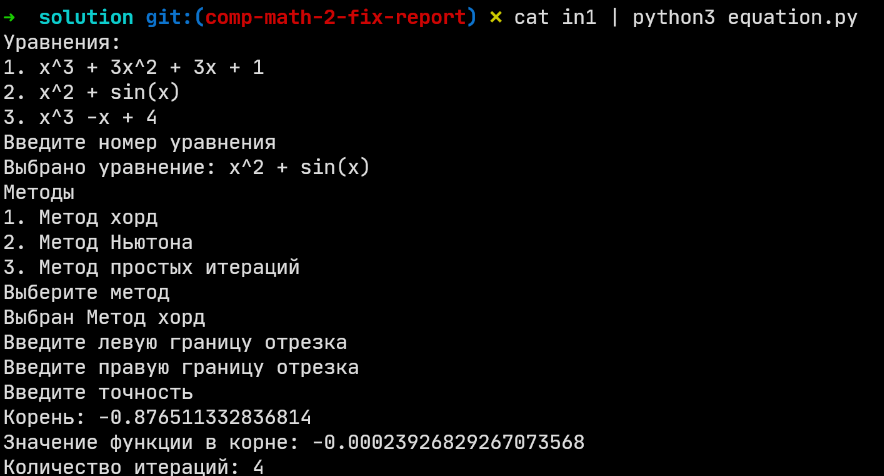
\includegraphics[width=0.9\textwidth]{./img/test1.png}
\end{figure}

\begin{figure}[H]
	\centering
	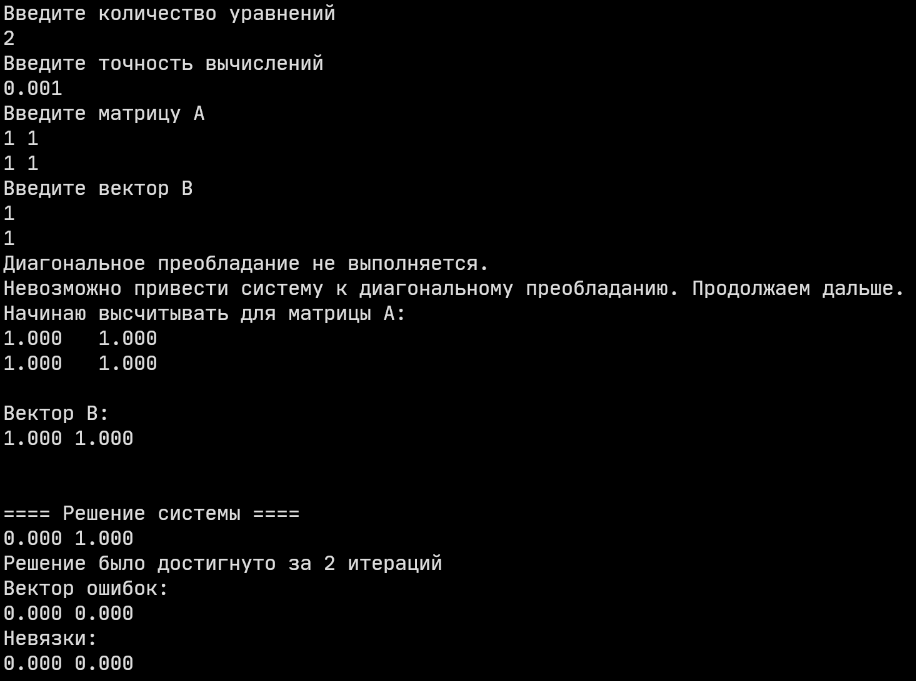
\includegraphics[width=0.9\textwidth]{./img/test2.png}
\end{figure}

\begin{figure}[H]
	\centering
	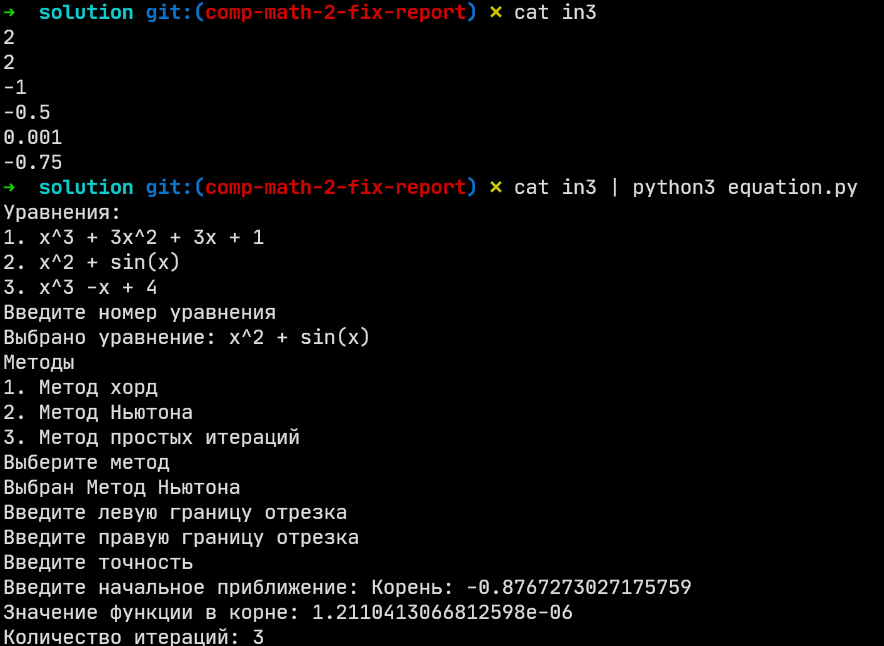
\includegraphics[width=0.9\textwidth]{./img/test3.png}
\end{figure}

\begin{figure}[H]
	\centering
	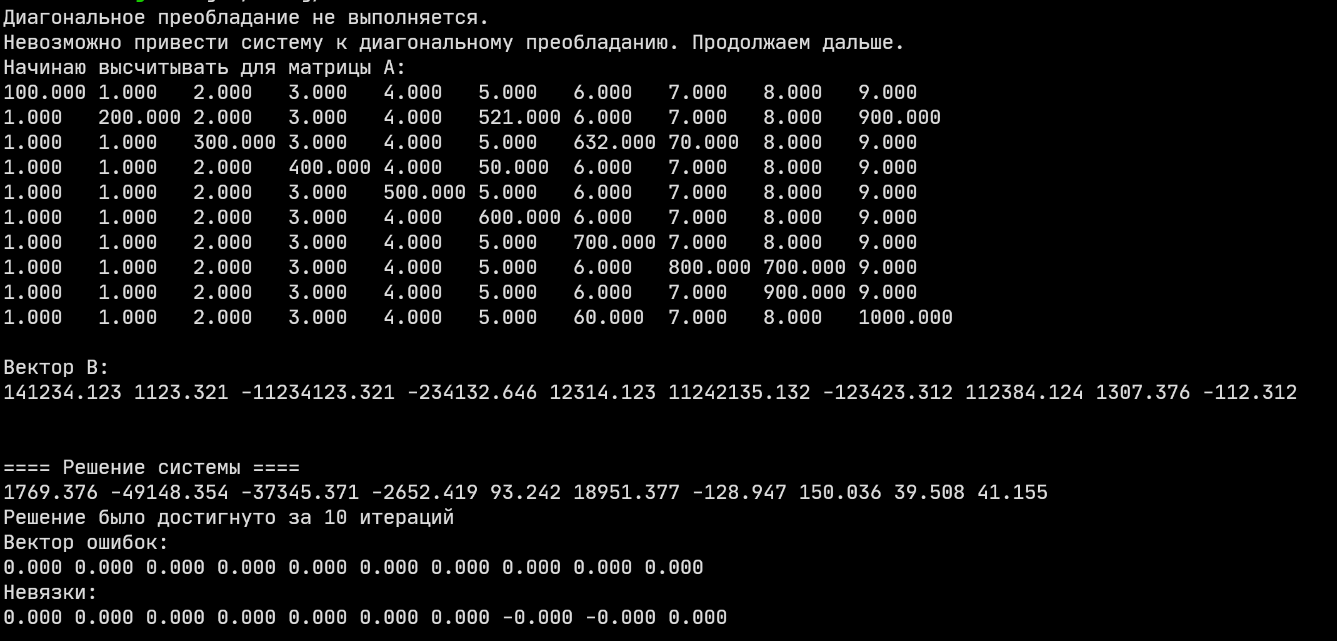
\includegraphics[width=0.9\textwidth]{./img/test4.png}
\end{figure}


\section{Вывод}
При выполнении данной лабораторной работы я изучил и программно реализовал такие методы
численного решения уравнений как: метод хорд, метод простых итераций, метод Ньютона и
метод Ньютона для решения систем уравнений.
